\documentclass[11pt]{article}
\usepackage{geometry}                
\geometry{letterpaper}                   

\usepackage{graphicx}
\usepackage{amssymb}
\usepackage{epstopdf}
\usepackage{natbib}
\usepackage{amssymb, amsmath}
\DeclareGraphicsRule{.tif}{png}{.png}{`convert #1 `dirname #1`/`basename #1 .tif`.png}

\usepackage{color}
\usepackage{xcolor}
\usepackage{colortbl}

\usepackage{pdfpages}

\usepackage{siunitx}

\usepackage{float}

%\usepackage[ngerman]{babel} %use this if you write you thesis in GERMAN!
\usepackage[utf8x]{inputenc}
%\usepackage[babel,german=swiss]{csquotes}
%\usepackage[backend=bibtex8]{biblatex}

\bibliographystyle{unsrt}

\usepackage{listings}

%\title{SIMonkey - Modelling social affiliation in gelada baboons}
%\author{Frank Grossenbacher, Derk Wild, Michael Heutschi, Sofia Zbinden}
%\date{December 2014} 

\begin{document}



\thispagestyle{empty}

\begin{center}
\includegraphics[width=5cm]{ETHlogo.pdf}

\bigskip


\bigskip


\bigskip


\LARGE{ 	Lecture with Computer Exercises:\\ }
\LARGE{ Modelling and Simulating Social Systems with MATLAB\\}

\bigskip

\bigskip

\small{Project Report}\\

\bigskip

\bigskip

\bigskip

\bigskip


\begin{tabular}{|c|}
\hline
\\
\textbf{\huge{SIMonkey}}\\
\textbf{\LARGE{Modelling social affiliation in gelada baboons}}\\
\\
\hline
\end{tabular}
\bigskip

\bigskip

\bigskip

\LARGE{Frank Grossenbacher\\ Derk Wild\\ Michael Heutschi\\ Sofia Zbinden}



\bigskip

\bigskip

\bigskip

\bigskip

\bigskip

\bigskip

\bigskip

\bigskip

Zurich\\
December 2014\\

\end{center}



\newpage

%%%%%%%%%%%%%%%%%%%%%%%%%%%%%%%%%%%%%%%%%%%%%%%%%

\newpage
%\section*{Agreement for free-download}
%\bigskip
%
%
%\bigskip
%
%
%\large We hereby agree to make our source code for this project freely available for download from the web pages of the SOMS chair. Furthermore, we assure that all source code is written by ourselves and is not violating any copyright restrictions.
%
%\begin{center}
%
%\bigskip
%
%
%\bigskip
%
%
%\begin{tabular}{@{}p{3.3cm}@{}p{6cm}@{}@{}p{6cm}@{}}
%\begin{minipage}{3cm}
%
%\end{minipage}
%&
%\begin{minipage}{6cm}
%\vspace{2mm} \large Frank Grossenbacher
%
% \vspace{\baselineskip}
%
%\end{minipage}
%&
%\begin{minipage}{6cm}
%
%\large Michael Heutschi
%
%\end{minipage}
%
%\\  \\&
%\begin{minipage}{6cm}
%\vspace{2mm} \large Derk Wild
%
% \vspace{\baselineskip}
%
%\end{minipage}
%&
%\begin{minipage}{6cm}
%
%\large Sofia Zbinden
%
%\end{minipage}
%\end{tabular}
%
%
%\end{center}
%\newpage


\includepdf{Photos/Agreementforfreedownload.pdf}
%%%%%%%%%%%%%%%%%%%%%%%%%%%%%%%%%%%%%%%



% IMPORTANT
% you MUST include the ETH declaration of originality here; it is available for download on the course website or at http://www.ethz.ch/faculty/exams/plagiarism/index_EN; it can be printed as pdf and should be filled out in handwriting
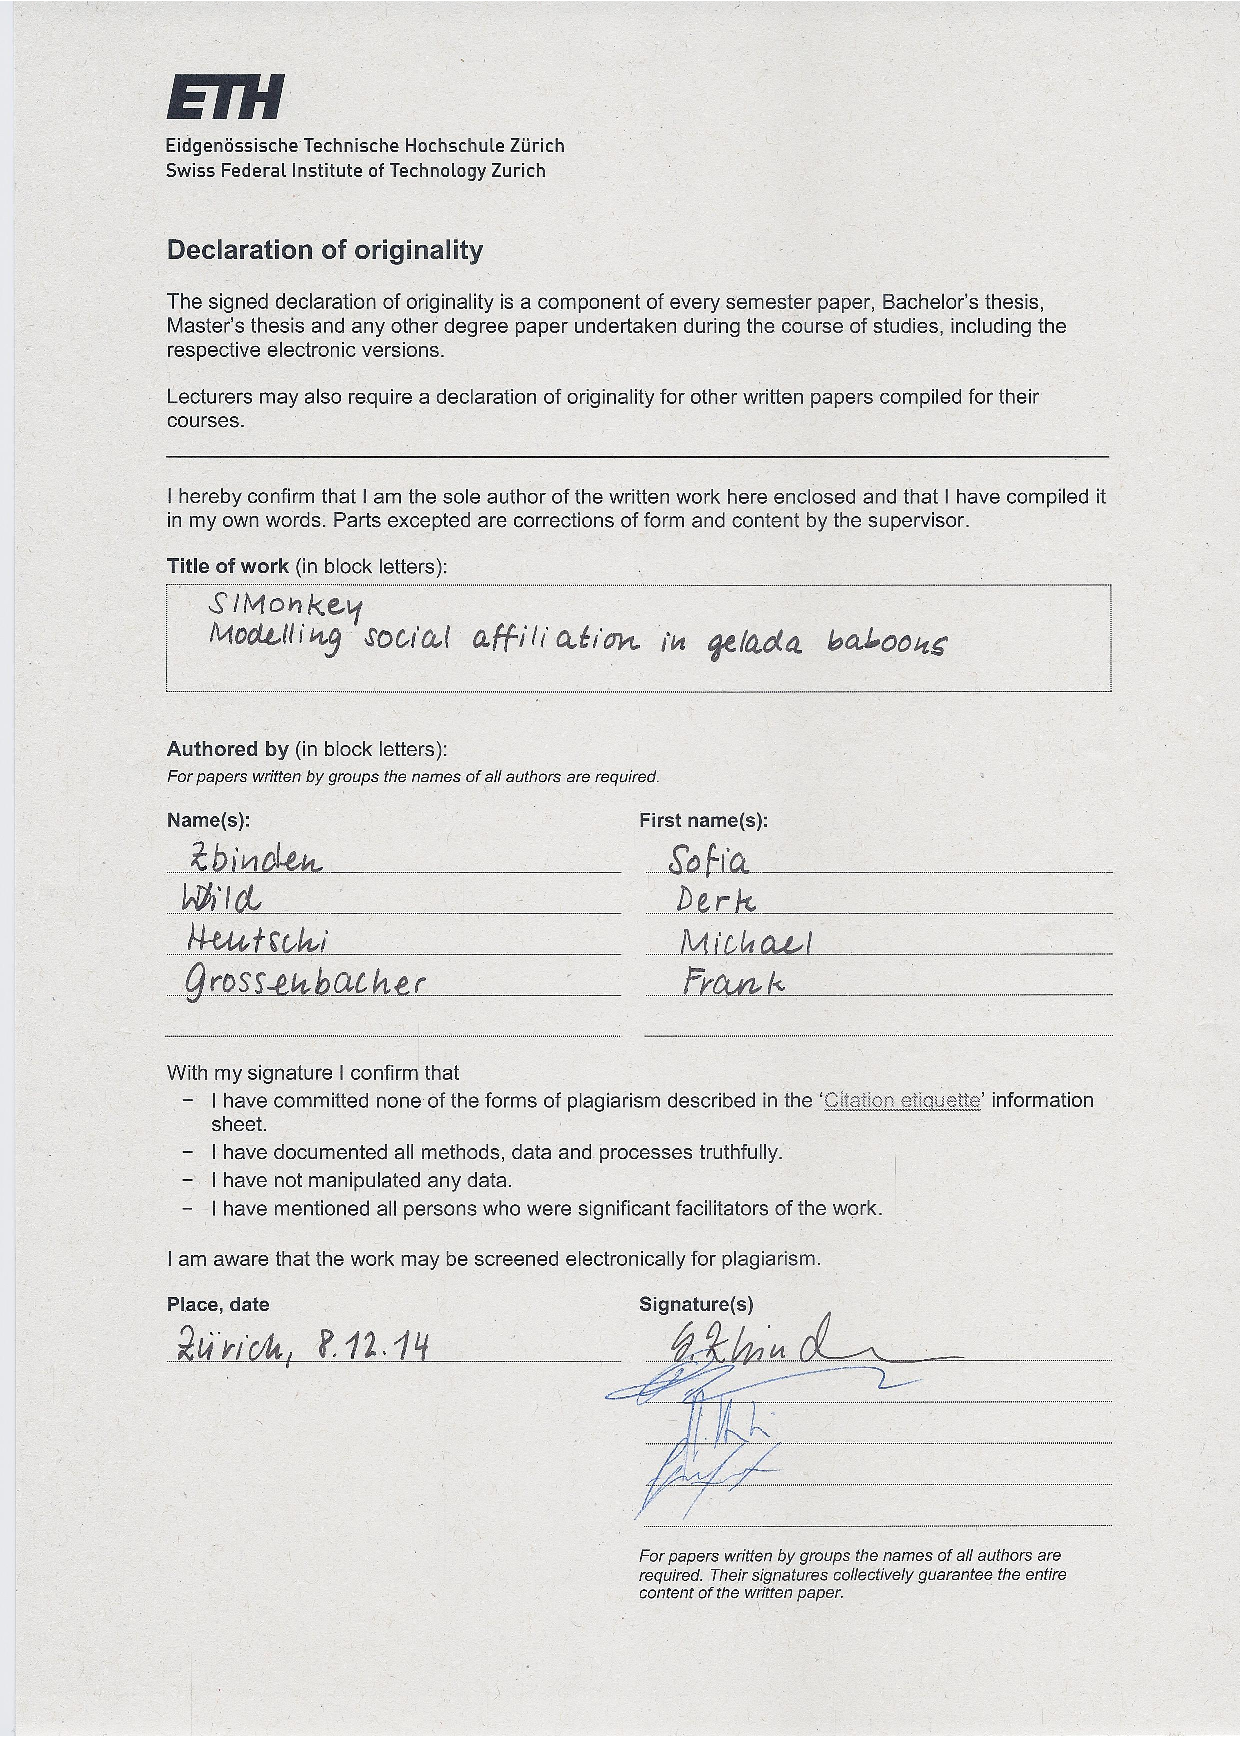
\includepdf{Photos/Declarationoforiginality.pdf}
%
\includegraphics[viewport=3.5cm 5cm 20cm 26cm]{declaration-originality}

%%%%%%%%%% Table of content %%%%%%%%%%%%%%%%%

\tableofcontents
\listoffigures

\newpage

%%%%%%%%%%%%%%%%%%%%%%%%%%%%%%%%%%%%%%%


%%%%%%%%%%%%%%%%%%%%%%%%%%%%%%%%%%%%%%%%%%%%%%%%%%%%%%%%%%%%%%%%%%%%%
% Abstract
%%%%%%%%%%%%%%%%%%%%%%%%%%%%%%%%%%%%%%%%%%%%%%%%%%%%%%%%%%%%%%%%%%%%%
\section{Abstract}
The social structure of gelada baboons is very interesting. Geladas form two different groups, a reproductive unit and an all-male group. In the reproductive unit are about one male and one to twelve females. The male often have one predominant female partner but can also interact with the others of its females. The females form strong social bonds and  a hierarchy in which closely related females tend to have the same hierarchical status\cite{Dunbar1974},\cite{Dunbar1980}.
\\
In this report we present a model to simulate social affiliation in monkeys, GrooFiWorld\cite{Puga-Gonzalez2009}. With this model as base we simulated the social structure of gelada baboons.\\
With the simulation we can show that it is possible to reduce the structure of social behaviour of gelada baboons to only four interactions for each baboon. Grooming, fighting, dominance and anxiety.


%%%%%%%%%%%%%%%%%%%%%%%%%%%%%%%%%%%%%%%%%%%%%%%%%%%%%%%%%%%%%%%%%%%%%
% Individual contributions
%%%%%%%%%%%%%%%%%%%%%%%%%%%%%%%%%%%%%%%%%%%%%%%%%%%%%%%%%%%%%%%%%%%%%
\section{Individual contributions}
As we are a group, we all worked together on this project. We had nearly every week a team meeting and discussed as much as possible together. But of course not every one can do everything, so we split the work as follows.\\
Derk Wild had most of the ideas what we can do and searched for good material to work on. In the end he also did programming work. Michael Heutschi and Frank Grossenbacher started with the first implementation of the model and developed the foundation of our code. They worked whole nights to enhance the code as good as we can. Me, Sofia Zbinden, I worked mostly on the report and did the organization of our group. 


%%%%%%%%%%%%%%%%%%%%%%%%%%%%%%%%%%%%%%%%%%%%%%%%%%%%%%%%%%%%%%%%%%%%%
% Introduction and Motivation
%%%%%%%%%%%%%%%%%%%%%%%%%%%%%%%%%%%%%%%%%%%%%%%%%%%%%%%%%%%%%%%%%%%%%
\section{Introduction and Motivations}
\subsection{Introduction: Social structure of gelada baboons}
\label{sec:Introduction}
Gelada baboons are very interesting and in their own way beautiful monkeys. They have long, grey and brown fur. The males are bigger than the females and have a red triangle on their chest (Figure \ref{fig:MaleGelada}).\\
Gelada baboons live in one of the most complex social structures among the whole animal kingdom. They form a so called multi level society where the females live in a harem with only one male in it (Figure \ref{fig:GeladaGroup}). This harem, called reproductive unit, contains one to twelve females. The rest of the male monkeys form pure male groups, the all-male groups\cite{Dunbar1986},\cite{Crook1966},\cite{Gruter2004}.\\
In the reproductive unit the male often have one predominant female partner, but it can also interact with its other females. But only the dominant female can monopolize the male if it wants. However it only does it if it has no alternative\cite{Dunbar1983}. This relationship between the male and its predominant female is similar to the especially relationship among the females. Very interesting are the  strong bonds the females build\cite{Dunbar1986}. They form a hierarchy in their group in which closely related females tend to have the same hierarchical status\cite{Dunbar1980}.\\
In the all-male groups they are some sub adults and one young adult. The young adult is led by one male of the group\cite{Dunbar1974}. Within the group aggression is not really remarkable, like in the reproductive units, but towards other groups there's lots of aggression based on the all-male group\cite{Dunbar1974},\cite{Dunbar1984}.\\
In the reproductive and the all-male unit grooming is a very frequent activity. It has several functions which are: cleaning the fur, reducing anxiety, tension and stress, social bonding, repairing relationships and social reciprocation and exchange\cite{Puga-Gonzalez2009}. Mostly grooming occurs between individuals of a similar rank because they have similar needs, but it occurs also between two former opponents after a fight\cite{Puga-Gonzalez2009}. After a fight the baboon of lower rank grooms the other one.\\
In every group some gelada baboons of similar hierarchical status have a very strong relationship. The quality of this relationship is influenced by security, value and the compatibility of both partners\cite{Puga-Gonzalez2009}. 

\begin{figure}[H]
\centering
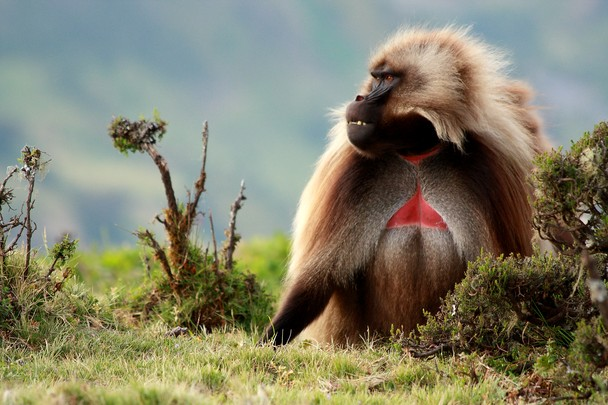
\includegraphics[scale=0.4]{Photos/NationalGeographic_BrianShuchuk}
\caption[Male gelada baboon]{Male Gelada Baboon in Simien Mountains, Ethiopia.
Source: National Geographic, Photo and caption by Brian Shuchuk: A moment captured during a trek in the Simien Mountains National Park, Ethiopia in November 2012.}
\label{fig:MaleGelada}
\end{figure}


\begin{figure}[H]
\centering
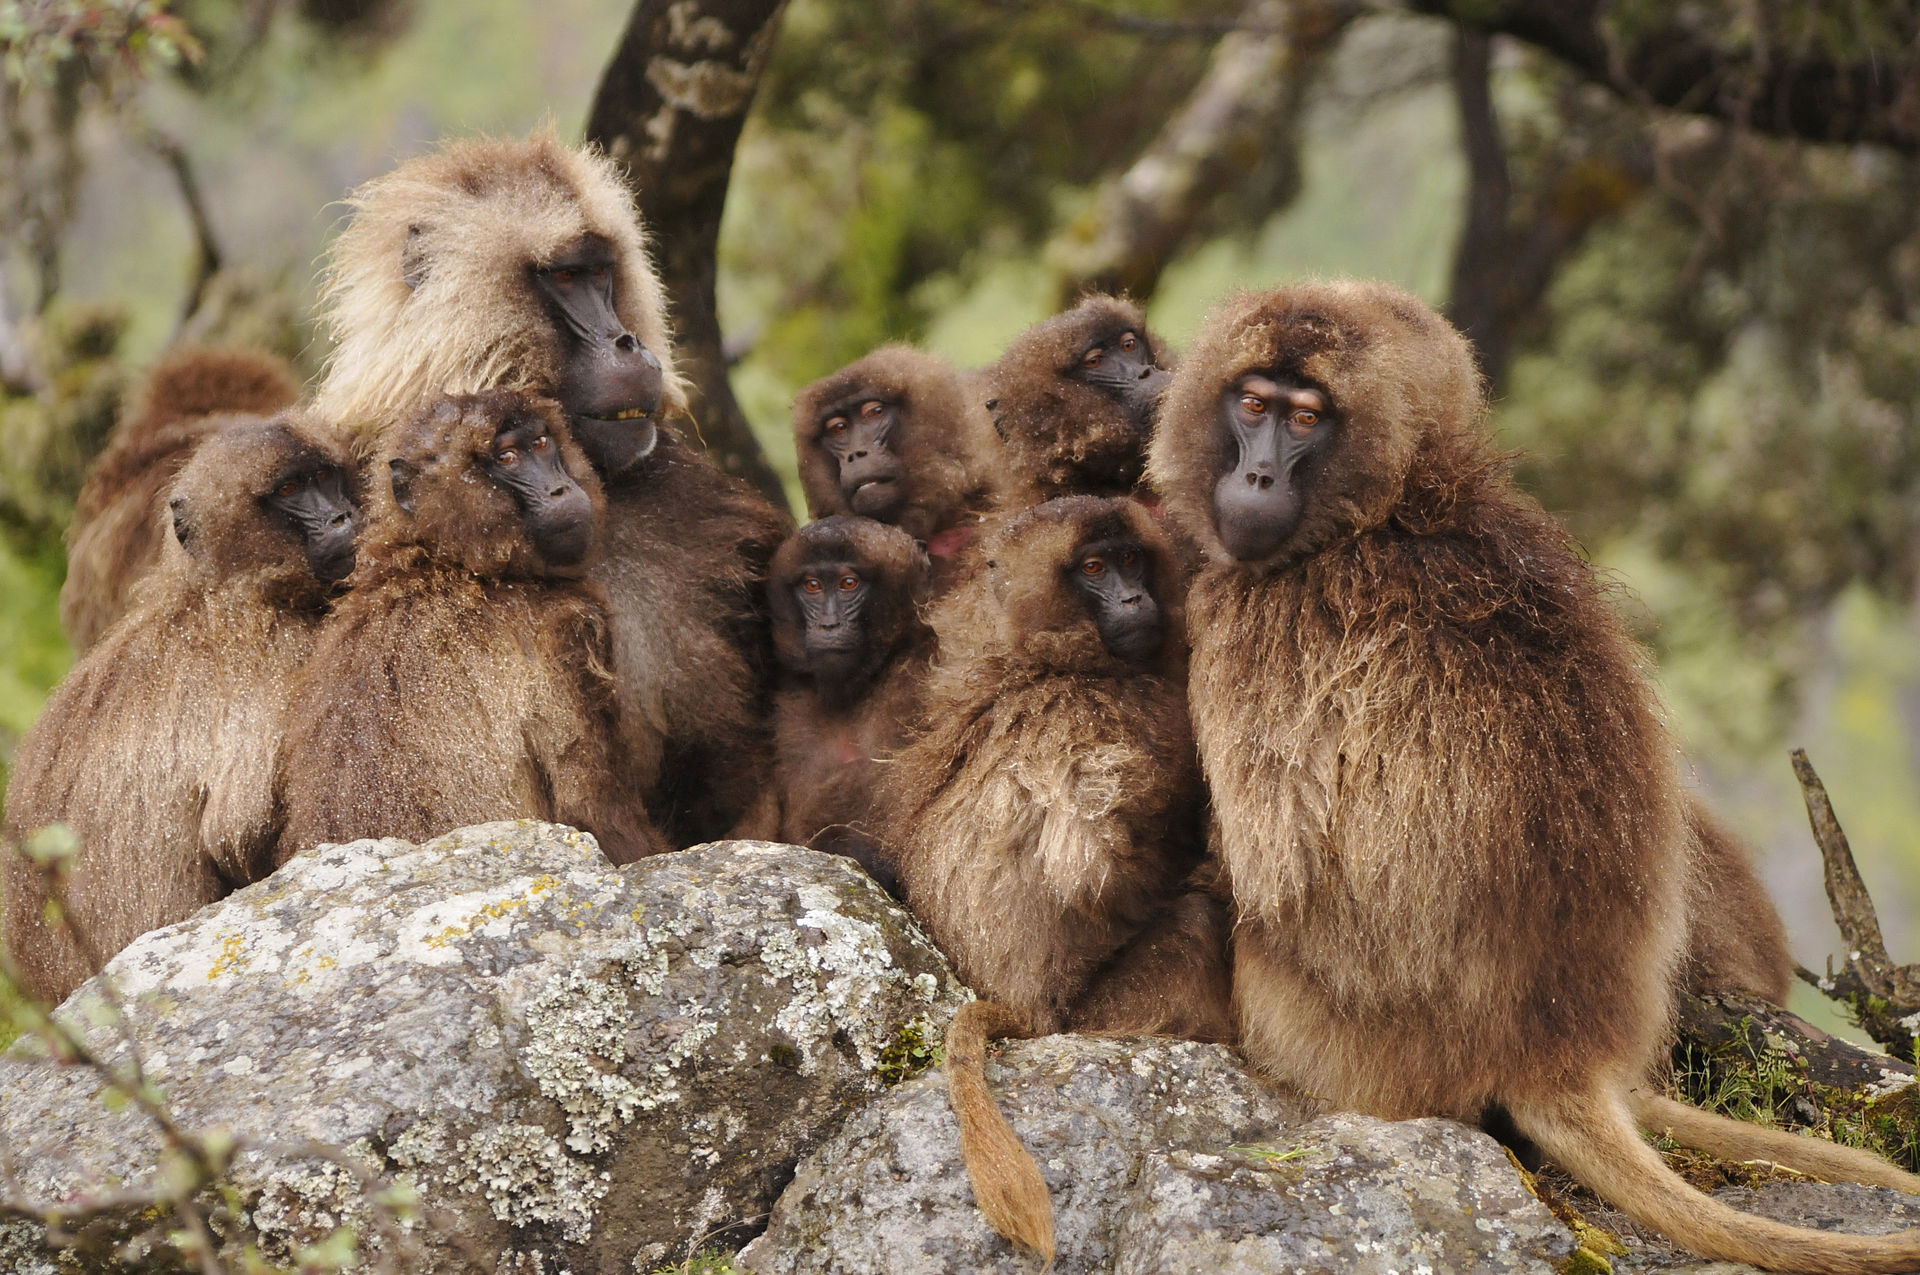
\includegraphics[scale=0.55]{Photos/Gelada_group}
\caption[Gelada reproductive unit]{Gelada reproductive unit. $http://en.wikipedia.org/wiki/Gelada (09.12.2014)$}
\label{fig:GeladaGroup}
\end{figure}

\begin{figure}[H]
\centering
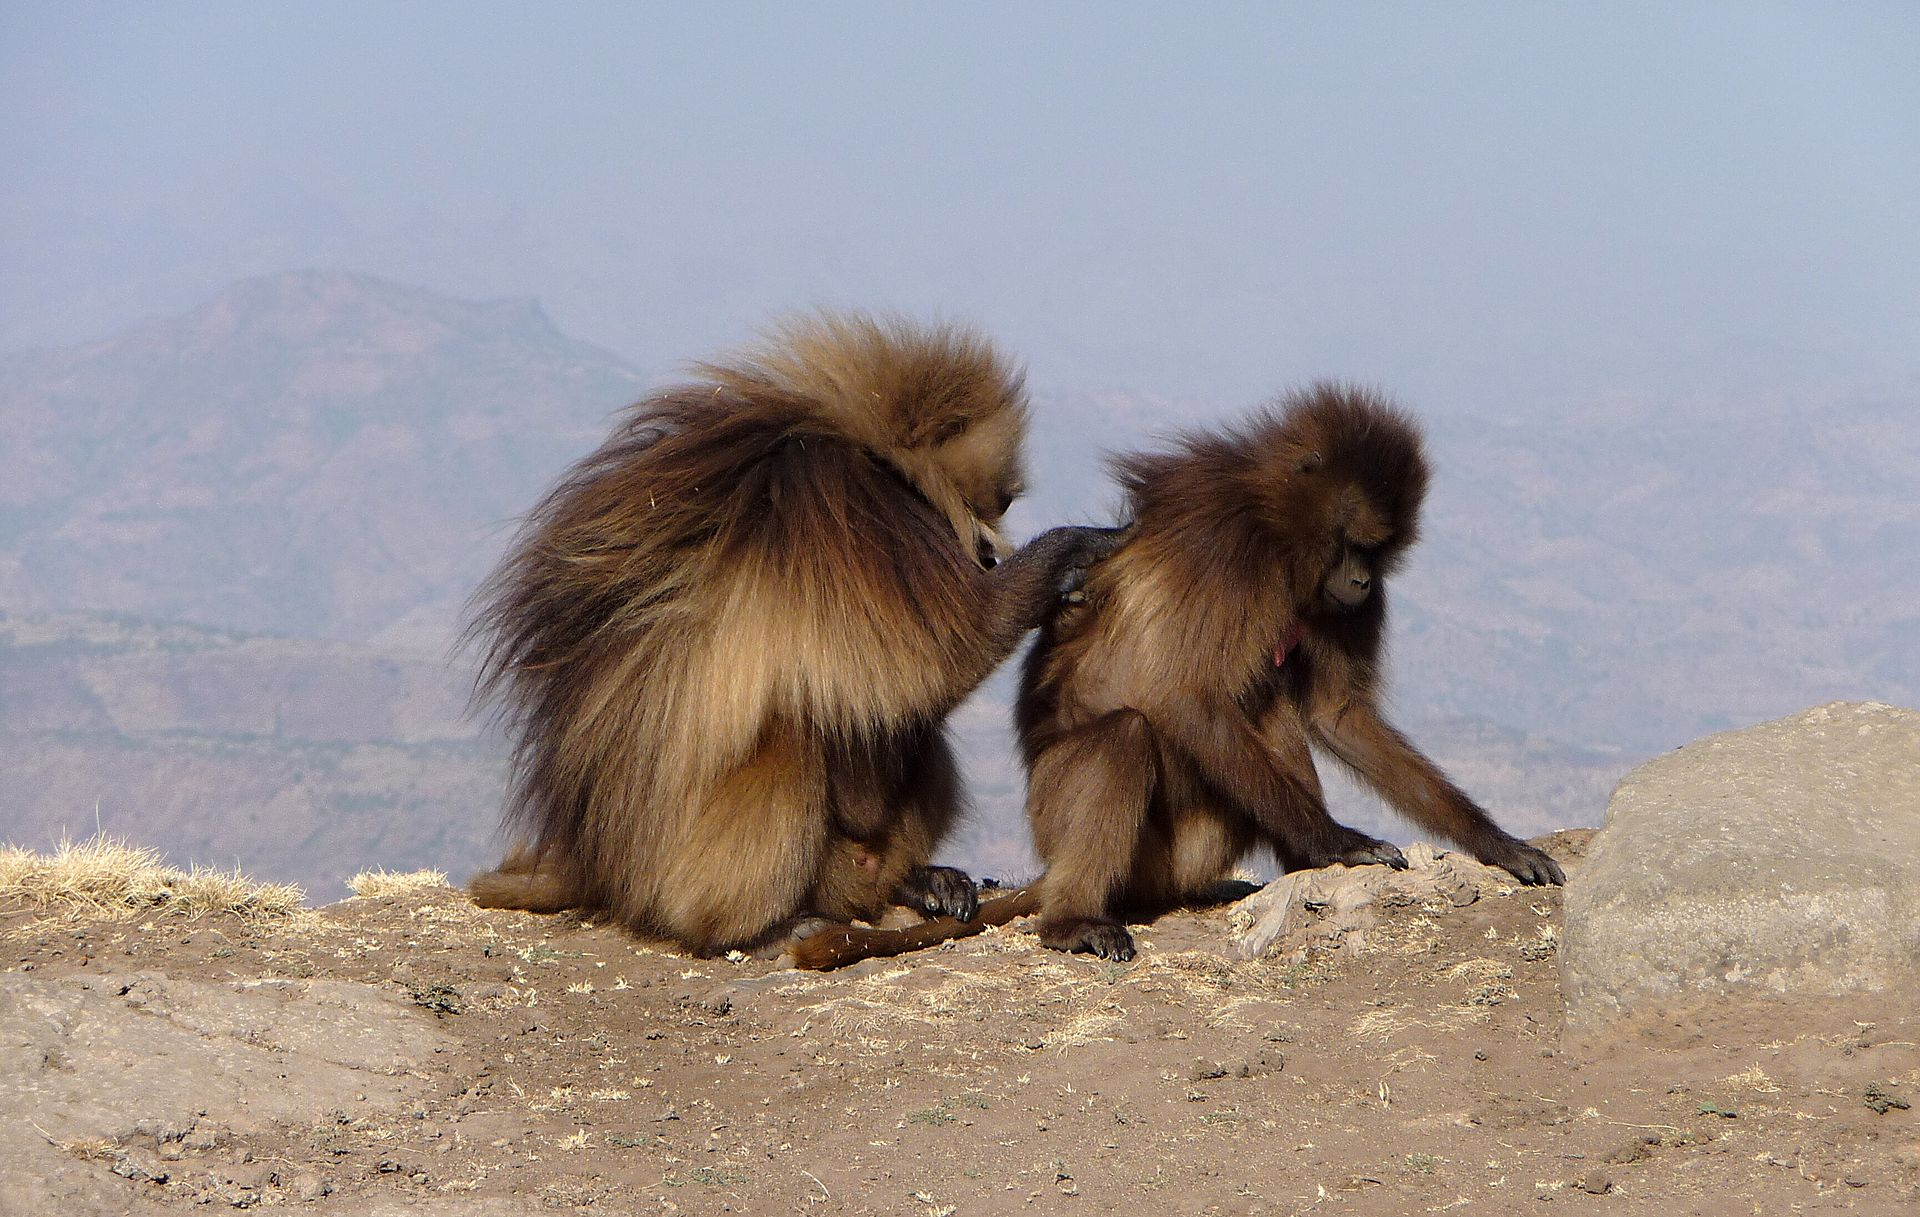
\includegraphics[scale=0.35]{Photos/Dzelady}
\caption[Male gelada grooming a female]{Male gelada grooming a female. $http://en.wikipedia.org/wiki/Gelada (09.12.2014)$}
\label{fig:Grooming}
\end{figure}

\subsection{Motivation}
\label{sec:Motivation}
As we searched for good, already existing models of the social structure of monkeys we found one that we can use for our project. The model we found is called GrooFiWorld and is published by Gonzalez et al. in 2009\cite{Puga-Gonzalez2009}. It's a model for 'emergent patterns of social affiliation in primates'\cite{Puga-Gonzalez2009}.
\\
We decided to take this model as a base and apply some changes to it to get a simulation of grouping of monkeys. We want to simulate the interesting social structure of the gelada baboons, to find out what are the important variables and parameters for the model and to get the grouping to a harem.\\
At the end our question is, if it's possible to get this form of grouping of females around one male if we only consider two variables for activities of the baboons and two variables of the well-being of the baboons.


%%%%%%%%%%%%%%%%%%%%%%%%%%%%%%%%%%%%%%%%%%%%%%%%%%%%%%%%%%%%%%%%%%%%%
% Description of the Model
%%%%%%%%%%%%%%%%%%%%%%%%%%%%%%%%%%%%%%%%%%%%%%%%%%%%%%%%%%%%%%%%%%%%%


\section{Description of the Model}
\subsection{GrooFiWorld}
As mentioned in section \ref{sec:Motivation} of this report, we used the model GrooFiWorld as base of our model. GrooFiWorld is an Agent-Based model written in C++\cite{Puga-Gonzalez2009}. The model is based on two frequent activities of monkeys. Grooming and fighting, as represented in it's name.\\
\[ \overbrace{\textbf{Groo}}^\text{grooming}\underbrace{\textbf{Fi}}_\text{fighting}\textbf{World} \]
The World is without any borders, it is continuous and the monkeys are free to move in any direction. The monkeys have a certain angle of vision in which they can see others and can interact with them.\\
The monkey's well-being  is displayed with theirs  dominance (DOM) and anxiety (ANX). When the monkeys groom, they reduce their own anxiety and are out of fear of being defeated. But also, grooming reduces the motivation to be groomed or to groom again. Not being groomed after some time increases the monkey's anxiety and increases their motivation to be groomed or to groom. Anxiety also changes with fighting. After a fight of two monkeys the anxiety is increased for both individuals.\\
When two individuals meet they first decide whether or not to attack. This decision depends on the dominance of the two. Higher dominance of the other monkey means higher risk of losing the fight. A fight is only initiated when an individual expects to win. If it expects to lose the individual makes a decision of grooming the other one. After a fight the anxiety grows for both individuals. The decision to go into a fight (mental fight) and the real fight are presented in equation \ref{eq:Fight}. This equation is based on the relative dominance of two monkeys (individual $i$ and individual $j$) and a random number between zero and one. If the result is $1$ the individual $i$ is a winner, else if the result is $0$ the individual $i$ loses.
\begin{equation}
\label{eq:Fight}
w_i=\left\lbrace\begin{array}{cc}
1 & ,\frac{\text{DOM}_i}{\text{DOM}_i+\text{DOM}_j}>\text{RAND}(0,1)\\
0 & ,\text{else}
\end{array}\right.
\end{equation}
After a fight the dominance values get updated presented in equation \ref{eq:DomUpdate1} for the monkey $i$ an in equation \ref{eq:DomUpdate2} for the monkey $j$. The value stepDom is a scaling factor for the dominance. It's between zero and one. The looser of the fight flees over a given distance in a random direction.
\begin{equation}
\label{eq:DomUpdate1}
\text{DOM}_i =\text{DOM}_i +(w_i -\frac{\text{DOM}_i}{\text{DOM}_i +\text{DOM}_j})\cdot\text{stepDOM}
\end{equation}
\begin{equation}
\label{eq:DomUpdate2}
\text{DOM}_j =\text{DOM}_j -(w_i -\frac{\text{DOM}_j}{\text{DOM}_i +\text{DOM}_j})\cdot\text{stepDOM}
\end{equation}
When an individual made the decision not to fight, it makes the decision of grooming. The monkey makes this decision with it's present value of anxiety and a random value between zero and one. The monkey grooms if $ANX > \text{RAND(0,1)}$, else no interaction occurs.\\
During periods without grooming, periods of no interaction, the anxiety of the monkeys increases\cite{Puga-Gonzalez2009}.\\

Figure \ref{fig:GrooFiWorld} shows the structure of the model GrooFiWorld. It is split in interaction and grooming and shows all activities and decisions a monkey do in which order.

\begin{figure}[H]
\centering
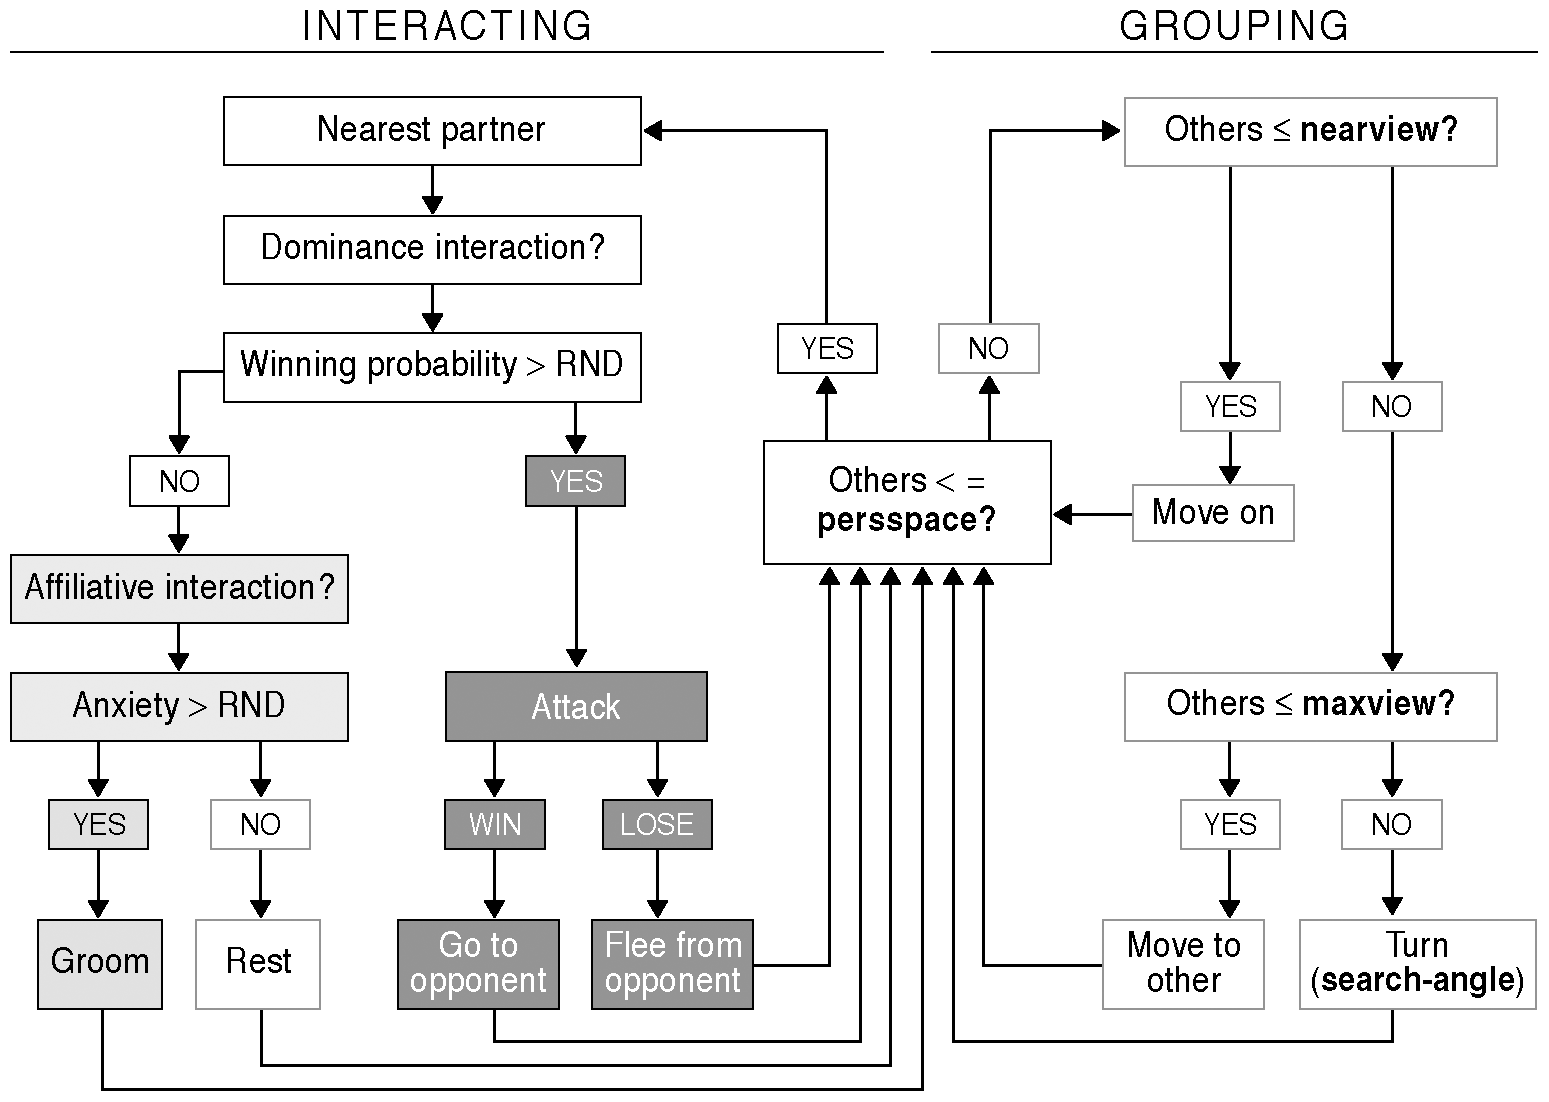
\includegraphics[scale=0.35]{Photos/Structure}
\caption[Structure of the model GrooFiWorld]{Structure of the model GrooFiWorld\cite{Puga-Gonzalez2009}}.
\label{fig:GrooFiWorld}
\end{figure}


\subsection{SIMonkey}
\label{sec:SIMonkey}
For our simulation a similar structure than used in GrooFiWorld was chosen. However, the program was simplified significantly by adding no directionality to the baboons so they have \SI{360}{\degree} view angle and movement. Therefore the structure had to be slightly changed to still achieve grouping. The Structure is shown in Figure \ref{fig:SIMonkey_Flussdiagramm}. The first addition is that an individual remembers with whom it just interacted and does not interact with that individual in the next round. This scheme enables grouping. A second addition to achieve harem like groups is the discrimination between alpha male and normal individuals. The alpha male behaves a bit different than the others. It seeks only for male individuals for interaction and since its dominance and therefore winning probability is the highest of all, it is likely to perform a fight and therefore chases the males within its view.

\begin{figure}[H]
\centering
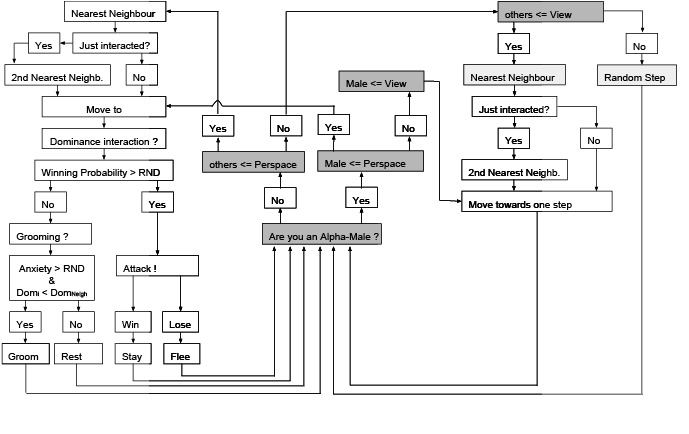
\includegraphics[scale=0.65]{Photos/Flussdiagramm}
\caption[Structure of the model SIMonkey]{Structure of the model SIMonkey.}
\label{fig:SIMonkey_Flussdiagramm}
\end{figure}

\section{Implementation}
The model is individual-oriented and event-driven. It has been written in Matlab R2014b and bases on vectorized variables. These variables sum the number of gelada baboons so that every individual is described precisely.
We used the model GrooFiWorld as base. But we implemented the whole code by ourselves new in Matlab. We used the ideas from the model and adopt some variables but choose new names.

\subsection{Structure of the Algorithm}
The structure of our algorithm is presented in Figure \ref{fig:structure}. First the initial and boundary conditions are set. Then there is a first loop over time and in this loop there is a loop over all baboons. The active baboon, individual $i$, first searches for the nearest baboon and checks if this baboon is near enough for an interaction. If yes, individual $i$ interacts with individual $j$. Else there's no interaction and the active baboon makes a random move. In the end the results get visualized in a plot.\\
\begin{figure}[H]
\centering
\frame{
\begin{tabular}{c}
\cellcolor{yellow}Set initial \& boundary conditions\\
\cellcolor{green!50}\textbf{Loop over time}\\
\cellcolor{green!50}\begin{tabular}{c}\cellcolor{green!85!black}\textbf{Loop over baboons}\\
\cellcolor{green!85!black}visualize inital position\\
\cellcolor{green!85!black}Baboon $i$ find other individual $j$ \& checks if it is in it's $view$\\
\cellcolor{green!85!black}\begin{tabular}{cc}
\cellcolor{red!50!black}found $j$ & \cellcolor{green!50!black}$j$ not found\\
\cellcolor{red!50!black}check if it's in interaction\_distance & \cellcolor{green!50!black}no interaction\\
\cellcolor{red!50!black}\begin{tabular}{c}\rowcolor{green!70!black}\textbf{Interaction $i$ with $j$}\\
\rowcolor{green!70!black}$i$ moves next to $j$\\
\rowcolor{green!70!black}Mental fight (twice)\\
\cellcolor{green!70!black}\begin{tabular}{cc}
\cellcolor{red!70}fight & \cellcolor{red!90!black}no fight\\
\cellcolor{red!70}increase $dom$ \& decrease $anx$ & \cellcolor{red!90!black}decision of grooming\\
\cellcolor{red!70}loser flees & \cellcolor{red!90!black}\begin{tabular}{cc}
\cellcolor{red!78!black}grooming & \cellcolor{red!90}no grooming\\
\cellcolor{red!78!black}decrease $anx$ & \cellcolor{red!90}increase $anx$\\
\cellcolor{red!78!black}$i$ and $j$ stay & \cellcolor{red!90}$i$ and $j$ stay
\end{tabular}\\
\cellcolor{red!70}winner stays & \cellcolor{red!90!black}
\end{tabular}\\
\cellcolor{green!70!black}
\end{tabular} & \cellcolor{green!50!black}move one step randomly\\
\cellcolor{red!50!black} & \cellcolor{green!50!black}decrease $dom$
\end{tabular}\\
\cellcolor{green!85!black}increase anxiety\\
\cellcolor{green!85!black}visualize interactions in main plot and statistics in subplots
\end{tabular}\\
\cellcolor{green!50}\\
\cellcolor{black!20}end
\end{tabular}
}
\caption[Structure of the algorithm]{Structure of the algorithm. A time loop in which there is a loop over all individuals and theirs interactions with each other.}
\label{fig:structure}
\end{figure}
The active individual~$i$ searches for the nearest other baboon. If a $nearest$ was found, the individual decides if it is either in interacting space, in sight or not. If ape~$nearest$ is close enough to the individual~$i$ a social interaction takes place. The interaction can be on the one hand fighting and on the other hand grooming. The decision whether to fight or not is calculated by the equation~ \ref{eq:DomUpdate1}. It is more possible that the active ape will attack if its relative dominance is higher than the others is. The same equation~\ref{eq:DomUpdate1} is also used to define the fight outgoing. So it's also possible that a weak baboon wins the fight but less supposable. The winner gets an increment in its victories and raises its dominance on a higher value and stays at its position. The loser decreases its dominance by the same amount.
If the individual~$i$ didn't decide to fight it will act as a groomer but only if its anxiety is higher than an random value (between 0 and 1) and its dominance is lower than the one of its partner. If this doesn't apply ape $i$ will rests at its present place and waits for the next round. But when it actually is entering the grooming section, the groomer~$i$ so as the groomee~$nearest$ reduces its anxiety value but it does so more strongly in the groomee. 
As described on the top its also possible that the active ape decides not to interact with anyone. One reason for that case could be, that no one is near enough or the decision equation~\ref{eq:DomUpdate1} calculated this possibility. If $no~interaction$ is elected the individual walks randomly around and updates its statistics. 
At the end of the code it will proof that none of the gelada baboons gets less dominance or anxiety values than zero and plots the final condition.



%%%%%%%%%%%%%%%%%%%%%%%%%%%%%%%%%%%%%%%%%%%%%%%%%%%%%%%%%%%%%%%%%%%%%
% Simulation Results and Discussion
%%%%%%%%%%%%%%%%%%%%%%%%%%%%%%%%%%%%%%%%%%%%%%%%%%%%%%%%%%%%%%%%%%%%%
\section{Simulation Results and Discussion}

On the Plot \ref{fig:Plot20} there are five subplots which shows what the individual apes are currently doing. On the main plot (left) is the map pictured where the gelada baboons are living. In real life that would be equal to \SI{900}{\meter\squared}. In the beginning the apes are scattered randomly in the black box (\SI{400}{\meter\squared}). The single dots represent the gelada baboons. Some of them are pink and the others are blue. The pink color shows which individuals are female and the blue which are male. Once the program is started the apes will walk around and maybe change their color. If their colors change the gelada baboons are interacting with each other. Every color represents a specific interaction between the activated partners (indicated by yellow). Green flashes up for a winner of a fight in opposite to a loser who's drawn as red. Orange and turquoise are set for a groomee and its groomer.

\begin{figure}
\label{fig:Plot20}
\centering
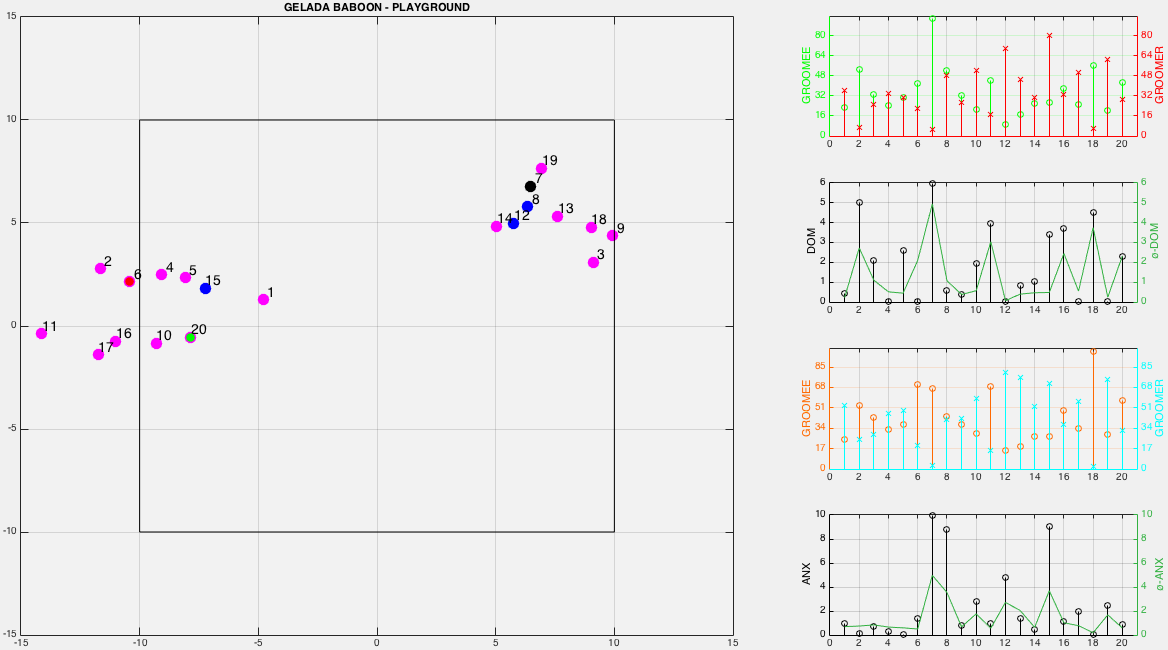
\includegraphics[scale=0.37]{Photos/mainplot_FG}
\caption{Main plot of the gelada baboon program}
\end{figure}

\begin{itemize} 
\item[violet:] The gelada grooms the other with slightly brighter violet, that means that it is getting groomed from the other.
\item[yellow:] There are always two apes which are yellow. What means, that they are interacting in this round. One of them will lose the fight, the other will win in the next round.
\item[red:] After the ape was yellow, and gets red, it stands for a lose in the past fight.
\item[green:] The opposite of the red color is the green one. Obviously it stands for the winner.
\end{itemize}
Beside on each dot is a number that numbers the gelada baboon and assign the dominance and the anxiety on the right side of the plot. After one round the statistic is updating and shows the present condition. So the user can, for example, follow which ape is the most powerful in one group and see if the they acting natural or if there are some parameter which should get changed. In the statistic is noticeable that there are always two colors in all four plots. The first one is similar to the the colors of of the dots. Green are the summed wins and red the summed losses of an ape. The second plot shows the current and the average dominance. It represents how strong the gelada is and let the user know if the ape rather lose or win in the next round. 
The third represent the groomee state of all. It has a direct influence to the anxiety which is plotted in the last field. The anxiety is equal built-on as the dominance plot. Black represent the present value and green the average of anxiety.\\
\\
Summarized the main plot \ref{fig:Plot20} displays the position and their activity of the apes. The statistic shows how strong each one of them are and represents rank in the group.

\section{Summary and Outlook}
\subsection{Summary}
\label{sec:Summary}
Our results from the simulation are very satisfying. The fundamental problem we confronted us with, to simulate baboons which form groups, is succeeded. The grouping is showed very good and we reached a simple but conceptional well representation of the simulation.\\
But there are some critical problems we want to point out here. The harem is not build as good we hoped to. We have the group building, but not always with only one male and the other females. This is the problem because we implemented that the baboon with the highest dominance is the alpha animal. In nature it's not only dominance that make up an alpha animal. In nature an animal with high dominance has first to fight against the present alpha animal and win against it.

\subsection{Outlook}
\label{sec:Outlook}
For the future it would be good to overwork the problem with the harem building. And in addition to that one could include directionality to the baboons so they have a view angle and can turn.

\subsection{Thanks}
We want to thank the whole MSSSM group of the chair of sociology, especially Tobias Kuhn and Olivia Woolley for their great help and good inputs.\\

\pagebreak
%%%%%%%%%%%%%%%%%%%%%%%%%%%%%%%%%%%%%%%%%%%%%%%%%%%%%%%%%%%%%%%%%%%%%
% References
%%%%%%%%%%%%%%%%%%%%%%%%%%%%%%%%%%%%%%%%%%%%%%%%%%%%%%%%%%%%%%%%%%%%%
\section{References}

\bibliography{bib/referencesSIMonkey}
\nocite{Dunbar1979}
\nocite{Dunbar1983}
\nocite{Dunbar1984}
\nocite{Dunbar1986}
\nocite{Crook1966}
\nocite{Kawai1983}
\nocite{Ohsawa1984}
\nocite{Gruter2004}

%%%%%%%%%%%%%%%%%%%%%%%%%%%%%%%%%%%%%%%%%%%%%%%%%%%%%%%%%%%%%%%%%%%%%
% Appendix
%%%%%%%%%%%%%%%%%%%%%%%%%%%%%%%%%%%%%%%%%%%%%%%%%%%%%%%%%%%%%%%%%%%%%
\newpage

\section{Appendix}
\subsection{MATLAB code}
\begin{lstlisting}[language=Matlab, backgroundcolor=\color{blue!10}, frame=single, framerule=0.1pt,commentstyle=\color{blue}, caption=main: SIMonkey\_live.m]

\end{lstlisting}

\begin{lstlisting}[language=Matlab, backgroundcolor=\color{blue!10}, frame=single, framerule=0.1pt,commentstyle=\color{blue}, caption=function: dist.m]
function [ dist ] = dist(xpos,ypos,i,j)

dist = norm([xpos(i),ypos(i)]-[xpos(j),ypos(j)]);

end
\end{lstlisting}

\begin{lstlisting}[language=Matlab, backgroundcolor=\color{blue!10}, frame=single, framerule=0.1pt,commentstyle=\color{blue}, caption=function: dommax.m]
function [ king ] = dommax(dom)

dom_j = dom(1);
nr_j = 1;
for j = 2:length(dom)
if dom(j) > dom_j
    dom_j = dom(j);
    nr_j = j;
    
end   
    
    king = nr_j;
end
\end{lstlisting}

\begin{lstlisting}[language=Matlab, backgroundcolor=\color{blue!10}, frame=single, framerule=0.1pt, commentstyle=\color{blue}, caption=function: move\_away\_random.m]
function [ coordinate_new ] = move_away_random(coordinate, 
flee_dist, direction)

% move towards point 0.5/0.5 when overshot 90% of field size
%if abs(0.5-x) > (f-0.5)*0.9
%    y = x+(0.5-x)*d;
% move randomly
%else
%    y = x+d*cos(2*pi*rand);
 %   while -f+1 > y || f < y
 coordinate_new = coordinate+flee_dist*direction;
 %   end
 
 % Fehlt:
 % Fluechte nicht zum feind HIN!
 % Fluechte nicht ueber feldrand!

end
\end{lstlisting}

\begin{lstlisting}[language=Matlab, backgroundcolor=\color{blue!10}, frame=single, framerule=0.1pt,commentstyle=\color{blue}, caption=function: plotall.m]
function [  ] = plotall(xpos,ypos,gender,spawning_size,
field_size,gela_nr,alpha)

% Plot whole Playground
subplot(1,3,1:2);
plot(xpos(1),ypos(1),'.','MarkerSize',40,'Color','w');
hold on;
for j = 1:length(xpos)
    if (gender(j) == 0 && alpha ~= j)                                     % females
      plot(xpos(j),ypos(j),'.','MarkerSize',40,'Color',
      '[1,0.4,0.9]');
    else if (gender(j) ~= 0 && alpha ~= j)                  
% normal males
      plot(xpos(j),ypos(j),'.','MarkerSize',40,'Color',
      '[0.1,0.3,0.8]');
        else                                                
% alpha male
        plot(xpos(j),ypos(j),'.','MarkerSize',40,'Color',
        '[1,0.8,0.4]');    
      
        end
    end
end
%hold off;
text(xpos(:),ypos(:),num2str(gela_nr),'VerticalAlignment',
'bottom', 'HorizontalAlignment','left','Color','k','FontSize',
14);           %'FontWeight','bold',
title('GELADA BABOON - PLAYGROUND');
grid on;
%bg = imread('grassland.jpg');  % Plot image as background
%imagesc(bg);
rectangle('Position',[-spawning_size/2,-spawning_size/2,
spawning_size,spawning_size]);
%text(-0.6,-0.1,int2str(n));
axis([-(field_size/2) (field_size/2) -(field_size/2) 
(field_size/2)]);  % set field size
hold off;

end
\end{lstlisting}

\begin{lstlisting}[language=Matlab, backgroundcolor=\color{blue!10}, frame=single, framerule=0.1pt,commentstyle=\color{blue}, caption=function: plotinteraction.m]
function [  ] = plotinteraction(gela_nr,xpos,ypos,gender,
alpha,spawning_size,field_size,i,nearest,interact_type)

% Plot whole Playground
subplot(1,3,1:2);
plot(xpos(1),ypos(1),'.','MarkerSize',40,'Color','w');
hold on;
for j = 1:length(xpos)
    if (gender(j) == 0 && alpha ~= j)                                     % females
      plot(xpos(j),ypos(j),'.','MarkerSize',40,'Color',
      '[1,0.4,0.9]');
    else if (gender(j) ~= 0 && alpha ~= j)                  
% normal males
      plot(xpos(j),ypos(j),'.','MarkerSize',40,'Color',
      '[0.1,0.3,0.8]');
        else                                                
% alpha male
        plot(xpos(j),ypos(j),'.','MarkerSize',40,'Color',
        '[1,0.8,0.4]');    
      
        end
    end
end
%hold off;
text(xpos(:),ypos(:),num2str(gela_nr),'VerticalAlignment',
'bottom', 'HorizontalAlignment','left','Color','k','FontSize',
14);           %'FontWeight','bold',
title('GELADA BABOON - PLAYGROUND');
grid on;
%bg = imread('grassland.jpg');  % Plot image as background
%imagesc(bg);
rectangle('Position',[-spawning_size/2,-spawning_size/2,
spawning_size,spawning_size]);
%text(-0.6,-0.1,int2str(n));
axis([-(field_size/2) (field_size/2) -(field_size/2) 
(field_size/2)]);  % set field size
hold off;

%Mark interacting Geladas with color
% interacting
if interact_type == 0
    hold on;
    plot(xpos(i), ypos(i),'.','MarkerSize',30,
    'MarkerEdgeColor','y');
    plot(xpos(nearest), ypos(nearest),'.','MarkerSize',30,
    'MarkerEdgeColor','y');
    hold off;

% i wins, nearest_gelada looses
elseif interact_type == 1
    hold on;
    plot(xpos(i), ypos(i),'.','MarkerSize',30,
    'MarkerEdgeColor','g');
    plot(xpos(nearest), ypos(nearest),'.','MarkerSize',30,
    'MarkerEdgeColor','r');
    hold off;

% nearest wins, i looses
elseif interact_type == 2
    hold on;
    plot(xpos(i), ypos(i),'.','MarkerSize',30,
    'MarkerEdgeColor','r');
    plot(xpos(nearest), ypos(nearest),'.','MarkerSize',30,
    'MarkerEdgeColor','g');
    hold off;

% i grooms nearest
elseif interact_type == 3
    hold on;
    plot(xpos(nearest), ypos(nearest),'.','MarkerSize',30,
    'MarkerEdgeColor','[0.5,0.1,0.9]');
    plot(xpos(i), ypos(i),'.','MarkerSize',30,
    'MarkerEdgeColor','[0.7,0.5,1]');
    hold off;
    
% nearest grooms i
elseif interact_type == 4
    hold on;
    plot(xpos(i), ypos(i),'.','MarkerSize',30,
    'MarkerEdgeColor','[0.5,0.1,0.9]');
    plot(xpos(nearest), ypos(nearest),'.','MarkerSize',30,
    'MarkerEdgeColor','[0.7,0.5,1]');
    hold off;
    
% doing a random walk
elseif interact_type == 5
    hold on;
    plot(xpos(i), ypos(i),'.','MarkerSize',30,
    'MarkerEdgeColor','b');
    hold off;

else
%do nothing
end

end
\end{lstlisting}

\begin{lstlisting}[language=Matlab, backgroundcolor=\color{blue!10}, frame=single, framerule=0.1pt,commentstyle=\color{blue}, caption=function: setminof.m]
function [ a ] = setminof( a,b )

% set minimum of dominance
if a < b
    a = b;
end
\end{lstlisting}

\begin{lstlisting}[language=Matlab, backgroundcolor=\color{blue!10}, frame=single, framerule=0.1pt,commentstyle=\color{blue}, caption=function: x\_move\_to\_individual.m]
function [ x_i_new ] = x_move_to_individual( x_i, y_i, 
x_neigh, y_neigh, displace)

%calculate distance btw the two baboons
dist = norm([x_neigh,y_neigh]-[x_i,y_i]);

%calculate x component of the normalized vector pointing 
%from i to nearest neighbour)
delta_x = (x_neigh - x_i)/dist;

%calculate x component of move vector(so that i is 'displace' 
%away from neighbour)
displ_x = delta_x*(dist-displace);

% new x coordinate (old coordinate + displacement)
x_i_new = x_i + displ_x;
end
\end{lstlisting}

\begin{lstlisting}[language=Matlab, backgroundcolor=\color{blue!10}, frame=single, framerule=0.1pt,commentstyle=\color{blue}, caption=function: y\_move\_to\_individual.m]
function [ y_i_new ] = y_move_to_individual( x_i, y_i, 
x_neigh, y_neigh, displace)

%calculate distance btw the two baboons
dist = norm([x_neigh,y_neigh]-[x_i,y_i]);

%calculate y component of the normalized vector pointing 
%from i to nearest neighbour)
delta_y = (y_neigh - y_i)/dist;

%calculate y component of move vector(so that i is 'displace' 
%away from neighbour)
displ_y = delta_y*(dist-displace);

%new y coordinate (old coordinate + displacement)
y_i_new = y_i+displ_y;
end
\end{lstlisting}

\end{document} 